\chapter{Methods}
% This should be 3000 words split with the results
% Probably gonna go for like 2200/800 as you have very few results

% the design of the task

%%%%%%%%%%%%%%%%%%%%%%%%%%
\section{Examining and Bridging the Gap}
\subsection{A Typical Decision Neuroscience Task}
% Two alternative forced choice
A typical decision neuroscience task involves the processing and accumulation of sensory evidence to trigger appropriate responses. The dot task discussed in the literature review is a discrete perceptual task requiring the subject to discriminate between one of two choices. This type of task can be broadly described as a "two-alternative forced choice" (2AFC) task. The 2AFC paradigm is the best understood and most commonly modelled type of task. The crux of this thesis was to fit driving to this paradigm where practicable; how can the complex task of driving be reduced in complexity to allow for effective modelling of the driver/cyclist interaction without sacrificing the ability to gain true insight into the decision process. Further to this, how could this 2AFC paradigm be approximated in such a way where it was still possible to capture additional complexity outside of its rigid, binary bounds. This crux was dubbed 'the Gap' which needed to be bridged between the two paradigms.

The first step in bridging the gap was to examine what the essential differences between either side were. This involved a significant period of discussion, research and attempts to work with previous trial data and models. The aim being to provide a strong framework to begin the design of the task in order to allow for the future modelling that was anticipated.

% what makes driving very complicated
\subsection{Driving as a Decision Task}
As discussed, driving is an incredibly complex task. It requires a constant monitoring of a wide variety of stimuli and near constant decision making. The depth, variety and complexity of these decisions can arguably be seen in the ongoing failures to implement self-driving cars. It is near impossible to comprehensively model the required environment and to then determine the 'correct' behaviour required for safe operation of a motor vehicle \citep{wolmarDriverlessCarsRoad2020}. Therefore, trying to fit this situation to the typical discretised and tightly controlled DN task requires some movement from both sides of the 'gap'. To facilitate this, the differences, similarities and bridging measures were discussed, detailed and examined. A summarisation of this work can be seen below in table \ref{tab:gap}.

\citep{wolmarDriverlessCarsRoad2020}

\begin{table}[H]
    \begin{center}
        \caption{Summary of 'the Gap'}
        \label{tab:gap}
        \resizebox{\textwidth}{!} {
        \begin{tabular}{p{0.3\textwidth}|p{0.3\textwidth}|p{0.3\textwidth}}
        \hline
        Typical Decision Science Task & Typical Driving Decision & 'Bridging' Measure \\ \hline
        Discrete \& binary decisions at known intervals & Continuous monitoring of a variety of stimuli \& decisions & Create a continuous monitoring framework which discretises the decision making process \\ \hline
        Subject has no control over the pace at which decisions occur   & Driver in total control of their speed and by proxy their decision rate  & Allow the subject to have control over their decision rate through a speed parameter \\\hline
        Two alternative forced choice decision paradigm  & Multi-factored decision process with an infinite number of choice combinations  & Design and implement task that captures the main contingencies and events of driving, but with reduced sensory and action alternatives and modelable 2AFC elements\\\hline
        Consequences for mistakes are minimal & Severe consequences for mistakes  & Provide feedback to the subject to discourage errors\\ \hline
        \end{tabular}}
    \end{center}
\end{table}

The remainder of this methodology chapter will discuss how this 'gap' was approached, what mitigating measures were implemented and how successful they were.

\section{Gaining Familiarity with Decision Neuroscience}
The modelling tools of DN rely on a depth of data to fit to, as aforementioned. To gain an understanding of how this depth of data is recorded, processed and analysed an examination of previous tasks was required. The cognitive neural systems lab has produced an enormous amount of data and associated models throughout its time in operation. It was decided that to gain this required understanding, an attempt would be made to fit a recently developed model from \citet{geuzebroekBalancingTrueFalse2023} to a previous dataset from \citet{kellyInternalExternalInfluences2013}. The reasoning was based on the continuous monitoring nature of the dataset which had been analysed as discrete in the 2013 paper. It was hoped that the continuous model from the more recent paper would be able to more completely capture the complexity of the dataset. While the model fitting was ultimately not completed the experience of exploring its application particularly with reference to the data handling methods, model design and task data output was invaluable for designing this thesis' task.

%%%%%%%%%%%%%%%%%%%%%%%%%%
\section{Beginning the Task Construction - Psychtoolbox, OpenGL and Perspective}
At the onset of this package of work a few key specifications were identified for the design of the task. In order to approximate the situation where compulsive overtaking had been observed the following were required:
\begin{itemize}
    \item A 3D representation of a road that was recognisable, but didn't contain any additional, unnecessary features.
    \item Randomly occurring cyclist objects
    \item An element of danger, oncoming traffic and cars 
    \item The ability for the subject to control the speed of their motion.
    \item The choice to slow down or to overtake when a cyclist appeared
    \item Some restriction on visibility. It must be possible for subjects to be surprised by the appearance of an object. 
\end{itemize}

% Why Psychtoolbox
Psychtoolbox is a software package created to form a bridge between MATLAB and computer display hardware \citep{kleinerWhatNewPsychtoolbox32007}. It allows incredible control over every pixel on the screen in a precisely timed frame by frame fashion. It is a standard software used within not just the cognitive neural systems lab in UCD, but also in DN research around the world. Furthermore, it builds upon the MATLAB workspace, familiar to UCD engineering students due to extensive use in the undergraduate and postgraduate engineering courses.

One of the earliest and largest challenges that was faced with the implementation of the decided upon task was Psychtoolbox's inability to handle perspective natively. While it is very capable of accurately drawing a variety of shapes to the screen with precise control over positioning it has no ability to handle the intricacies of camera projection similar to that seen in figure \ref{fig:MET_Projection}.

\begin{figure}[H]
    \centering
    \includegraphics[width=0.75\linewidth]{figures/Projection Diagram.png}
    \caption{Diagram showing the 'real frame' and its projection onto the display screen}
    \label{fig:MET_Projection}
\end{figure}

The early experimentation that took place in this project involved drawing a box to a screen which could imitate a 'cyclist' on the road as can be seen in figure \ref{fig:EarlyPsychExp}. This experimentation involved the rudimentary projection of a 'real frame' path taken by the cyclist onto a screen. It quickly became clear that the implementation of this projection by calculating the vector mathematics would require vastly more time and expertise in computer graphics than available. On top of this, limitations within MATLAB's processing efficiency would have made an implementation impractical. As a result, the task would have to make use of a different method.

\begin{figure}[H]
    \centering
    \includegraphics[width=0.45\linewidth]{figures/Slide1.png} \hfill
    \includegraphics[width=0.45\linewidth]{figures/Slide2.png}
    \caption{The Results of Early Experimentation in Psychtoolbox, a Square Which Appears to Move Closer to the Camera}
    \label{fig:EarlyPsychExp}
\end{figure}

% Talk about OpenGL
Thankfully, Psychtoolbox has a port of OpenGL, a application programming interface (API) which has extensive tools for rendering 3D graphics. However, it is quite a low-level interface, difficult to use without a strong foundation in C++ and computer graphics. The process of learning how to use the API took quite some time and was thankfully aided by an excellent book on the topic containing a step-by-step explanation of the rendering process \citep{vriesLearnOpenGLGraphics2020a}. The port of this API into Psychtoolbox is poorly documented, but there are some useful tutorials available on the internet in particular in the work of \citet{scarfeVisionHapticsLaboratory2023}.

Ultimately an adapted version of the general graphics pipeline was adopted. All concerns of lighting and texturing were abandoned for the sake of simplicity and to reduce the computational load that was quickly becoming apparent due to the inherent inefficiencies of using a port of an API, within a toolbox, within MATLAB. The objects which represent the road users are cubes with 8 vertexes drawn with specified dimensions which can be found in appendix \ref{tab:Dimensions}. Those vertexes are then translated to their calculated current positions using native OpenGL capabilities. The cyclist objects are drawn as green cubes and the car objects as red cubes. A diagram of this can be seen in \ref{fig:MET_Pos}. The road and centre lines on the other hand are 'Quad' objects drawn as flat planes along the ground.

% Talk about what this enabled
% Make particular note of how it enabled the use of units which have 1:1, useful correlation with the physical quantities we are looking to 
\begin{figure}[H]
    \centering
    \includegraphics[width=0.45\linewidth]{figures/MET_Positioning.png}
    \caption{Diagram Showing the 'Virtual Frame' Containing the Objects of Interest. Of Particular Import is the Co-Ordinate System Detailed.}
    \label{fig:MET_Pos}
\end{figure}

One of the great advantages of this approach was that objects' positions, speeds and sizes can be described using actual physical quantities and co-ordinates as seen in \ref{fig:MET_Pos}. That is opposed to the native Psychtoolbox approach which uses measurements relative to the screen in pixels. This proved to be of immense import, especially when it came to the implementation of motion, simplifying the complexity of the process significantly.

% Talk about camera & positioning
\begin{figure}[H]
    \centering
    \includegraphics[width=0.45\linewidth]{figures/Camera Positioning.png}
    \caption{Diagram describing how camera positioning is handled within OpenGL}
    \label{fig:CameraPos}
\end{figure}

OpenGL requires the placement of a camera in the virtual frame of reference, an explanation of which can be seen in \ref{fig:CameraPos}. It is this camera object which natively handles the projection of the scene in the virtual frame onto the screen's plane for display. With this fundamental framework established it was time to determine how and what to display and what factors to examine.

%%%%%%%%%%%%%%%%%%%%%%%%%%
\section{Constructing the Task Frame}
Control over the positioning and movement of objects within the 'real frame' without having to concurrently conduct complex vector and perspective calculations had been the primary motivation of the switch to OpenGL. Once that switch had been made the motion frame of the task had to be constructed. 

\subsection{Moving to a Relative Frame}
The 'virtual frame' previously seen in figure \ref{fig:MET_Pos} referred to here as the road, can be represented from above as in panel a) of figure \ref{fig:Frame Comparison}. The objects in this representation are moving as traffic moves in reality. The cyclist and car in the lane of the camera are moving with it and the traffic in the opposing lane is moving towards the camera. An important step in the creation of the task was the conversion of the motion of the 'driver' (represented by the camera) moving forward in the left lane to a relative frame seen in panel b) of figure \ref{fig:Frame Comparison}. The relative frame allowed all other road users represented in the task to be moved only with reference to the camera.

\begin{figure}[H]
    \centering
    \includegraphics[width=0.45\linewidth]{figures/Frame1.png} \hfill
    \includegraphics[width=0.45\linewidth]{figures/Frame2.png}
    \caption{The conversion from a) the 'real frame' of motion to b) the relative frame of motion}
    \label{fig:Frame Comparison}
\end{figure}

\subsection{Road Dimensions}
% Talk about centre lines
The dimensions of the road drawn on the screen correspond to the design standards of a typical Irish 'local road', contained within \citet{dotDesignManualUrban2013}. Those values are tabulated below:
\begin{table}[H]
    \begin{center}
        \caption{Tabulated Values of Road Dimensions From \citep{dotDesignManualUrban2013}}
        \begin{tabular}{cc}\hline
            Dimension       &   Value (m)   \\\hline
            Lane Width      &   2.5     \\
            Line Length     &   3.0     \\
            Line Gap        &   6.0     \\\hline
        \end{tabular}
    \end{center}
\end{table}

Every part of this setup is designed to maximise the familiarity of the subject to their environment without adding additional unnecessary distracting features which may influence their behaviour beyond what is appropriate for this study.

The inclusion of the centre lines is a significantly more important addition than would seem at first glance. Their motion is vital for the subject to be able to gather an intuitive sense of their speed during periods where there may not be any additional objects on the screen.
%%%%%%%%%%%%%%%%%%%%%%%%%%
\section{View Distance}
More possibilities emerged with the introduction of OpenGL as a framework through which to process perspective. One dynamic that came up frequently in discussion within the context of the driver/cyclist interaction was the overtaking of a cyclist despite an upcoming red light. Frequently a cyclist will be overtaken at a near distance only to immediately pass on the inside of the overtaking vehicle. Within the realm of work done by computer graphic professionals, a traffic light does not represent an object of immense complexity. However, within the context of the framework of this task it was deemed to be an inappropriate and overly complicated addition. This task was built upon the idea that subjects be shown a continuously varying and pseudo-randomly generated environment. Each level of complexity which gets added to this environment inevitably leads to additional edge cases, making it more difficult to be confident in the behavioural data extracted.

% Talk about how we scraped the continuous varying part of it
In order to examine the setting of different risk thresholds in a more controlled manner, use was made of an inherent feature of the OpenGL camera object, the draw distance. The draw distance is the distance from the camera that OpenGL will render objects, known further in this document as the 'View Distance' of the driver. A diagram describing this quantity can be seen in figure \ref{fig:ViewDist}

\begin{figure}[H]
    \centering
    \includegraphics[width=0.45\linewidth]{figures/Camera Viewing.png}
    \caption{Diagram Describing How 'View Distance' is represented in the Task}
    \label{fig:ViewDist}
\end{figure}

In the task, the view distance could take on one of three values, [20, 40, 80] meters. Following the end of a stimulus the view distance would smoothly adjust to a randomly chosen one of those values. After the adjust was complete the subjects would be given an opportunity to re-adjust their speed. It was hypothesised that subjects would reduce their speed when the view distance was smaller as they would have less time to react to a given stimulus.

\subsection{Perceived Gap}
\label{MET:perceivedGap}
This is a subsection of the view distance parameter. The perceived gap is the distance that a subject can see in the right lane which is currently unoccupied by an object. This value is closely linked to the view distance as it is identical when there is no object in the right lane. A diagram showing this can be seen below in figure \ref{fig:MET_Gap1}.
\begin{figure}[H]
    \centering
    \includegraphics[width=0.4\linewidth]{figures/MET_Gap1.png}
    \includegraphics[width=0.4\linewidth]{figures/MET_Gap2.png}
    \caption{Diagram Showing the 'Perceived Gap' in the Right Lane}
    \label{fig:MET_Gap1}
\end{figure}


\section{Object Appearance and Variance}
\subsection{Pseudo-Random Generation of Stimulus Onset Position}
% Talking about the fish method
For the sake of this task there are functionally two values that represent stimulus position in the 'virtual frame'. The first of these values is a position along the total length of the trial. As the camera is 'moving' along the trial (in actuality everything is moving towards the camera) it will eventually reach the stimulus onset position. At this point the stimulus will 'turn on' and begin to move towards the camera from a distance which is the second position value, discussed further on.

The generation of the stimulus onset positions was handled via a pseudo-random approach. A poisson sampling regime was employed using the inbuilt MATLAB function 'poissrnd'. This method allowed the use of an underlying 'rate' of occurrence for the objects to appear along the path. These rate of occurrences can be found tabulated in appendix \ref{tab:SamplingRate}. This sampling approach was pseudo-random due to the requirement that objects do not begin within a certain distance of each other in order to ensure that each decision the subject must make is independent of the next.

At one point this underlying appearance rate was considered to be of potential interest with regard to subject behaviour as a method to distinguish between areas of 'higher' \& 'lower' traffic. However, it was concluded that within the bounds of appropriate experimentation time, subjects would not have time to adequately adjust to the different rate levels. This would make it prohibitively difficult to determine a meaningful relationship between the factor and response variables. 

\subsection{Start Distance from Camera}
The second position variable of interest is the start distance from camera. This is functionally a measure of where the object will appear on the screen after it passes its stimulus onset position. This did not vary in the car objects, but did in the cyclist object randomly between one of three levels: [20, 40, 60] meters. It was hypothesised that cyclists appearing at closer distances would likely result in a higher level of overtakes.

\section{Cyclist Speed}
% The speed of the cyclists change
One factor of interest, hypothosised to influence the behaviour of subjects was the speed at which the cyclist stimulus moved. To vary this factor, samples from a normal distribution of speeds was used with a mean of $14 km/h$ taken from a survey conducted by \citet{gintyWhyCyclingRight2009}, and a standard deviation of $3 km/h$

\section{The Choice - To Overtake or To Slow Down}
The major simplification of this task relative to its real world allegory is the use of the 2AFC paradigm. A pictorial representation of this paradigm can be seen in figure \ref{fig:MET_2AFC}. The decision was made to take a simplified version of a common occurrence: a driver encountering a cyclist from behind on a narrow, two-lane road. In this situation the driver has one of two choices. Either they slow down to the pace of the cyclist and wait for an appropriate time to overtake or for the cyclist to turn off the road or they choose to overtake. Each of these choices has an associated cost and benefit, which can be seen briefly described below in table \ref{tab:CBA}.

\begin{figure}[H]
    \centering
    \includegraphics[width=0.45\linewidth]{figures/Methods_2AFC.png}
    \caption{Pictorial Representation of the Task Simplification into a 2AFC Paradigm}
    \label{fig:MET_2AFC}
\end{figure}

\begin{table}[H]
    \begin{center}
        \caption{Summarised Cost/Benefit of Decision}
        \label{tab:CBA}
        \resizebox{\textwidth}{!} {
        \begin{tabular}{p{0.3\textwidth}|p{0.3\textwidth}|p{0.3\textwidth}}\hline
            Choice      &   Cost  & Benefit \\\hline
            Slow down   &   Uncertain length of delay to driver  & Increased safety for both the cyclist and the driver  \\ \hline
            Overtake    &   Increased risk of collision to the driver with oncoming traffic; increased danger to the cyclist &  An elimination of the potential delay caused by slowing down  \\ \hline
        \end{tabular}}
    \end{center}
\end{table}

An important distinction between the results of this decision is that they have both internal and external costs and benefits. The choice a driver makes does not just affect themselves, but also imposes a cost or benefit onto the cyclist. In the case of an overtake, the costs are not fixed. If a driver chooses to overtake at speed or at a close distance the risk is significantly higher than if they make the same choice at a further distance or lower speed. In aggregate in reality this further imposes an unseen societal cost, if overtake decisions are made more frequently in these 'riskier' situations fewer people will choose to cycle, eliminating the benefits of the practice discussed previously.

In the process of designing this task, observations were made of common situations in which overtake decisions may occur with little benefit to the driver. A frequent occurrence that was observed was a tendency to always overtake; a situation of particular note is where there is no time benefit to the driver to overtaking, such as when a red light, stop sign, or intersection is just ahead. It was hoped that the design of this task would reflect this effect which has dubbed the 'must get in front'(MGIF) heuristic in popular discourse, but has thus far been absent from the literature.

In order to mimic the real world more closely and to gather data about the response times of the subjects outside the binary choice framework an 'in-lane car' was added to the task. This is an obstacle that a subject cannot overtake and therefore must choose to slow down for.

\section{The Mechanics of The Decision}
This discretisation of the decision to be made was essential for the functioning of the task. It allowed for the creation of 'fixed' responses to user input from the task itself. These responses took two forms based on which choice was made. The actual result of both choices in a trial can be seen below in figure \ref{fig:MET_Speed_Changes}, but they are discussed in detail in the two sections further along.
\begin{figure}[H]
    \centering
    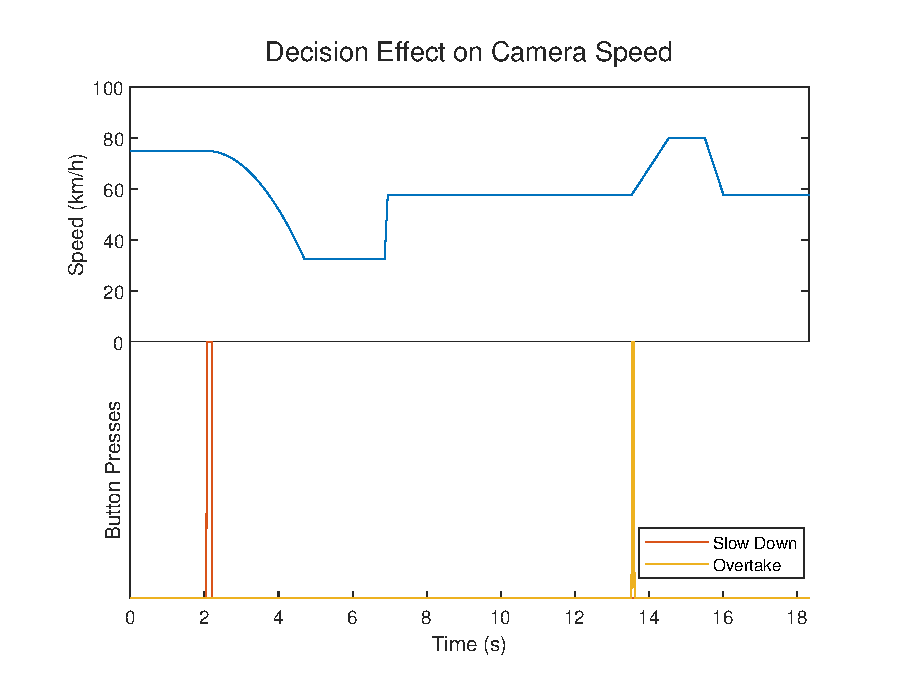
\includegraphics[width=0.6\linewidth]{figures/Method_Speed_Changes.eps}
    \caption{Plot Showing Changes in Camera Speed Following a Button Press}
    \label{fig:MET_Speed_Changes}
\end{figure}

\subsection{Overtaking}
The overtaking decision starts the subject on a path taking a fixed amount of time and moving the camera to simulate an overtaking manoeuver in reality. How this process is handled is shown in figure \ref{fig:MET_Over} and detailed step by step below.

\begin{figure}[H]
    \centering
    \includegraphics[width=\linewidth]{figures/Methods_Overtake.png}
    \caption{Diagram describing how the tasks handles the overtake decision in virtual space}
    \label{fig:MET_Over}
\end{figure}

The process of handling overtaking has 5 distinct steps. These are:
\begin{enumerate}
    \item The subject is continuing along at a steady pace. An object appears and the subject makes the decision to overtake.
    \item Following the decision being made, the subject clicks the right button and begins the process of overtaking at $t_{0}$. The camera moves its lateral $x$ position into the other lane and begins to accelerate at a fixed rate of $12 ms^{-2}$ for 1 second
    \item The camera reaches it's maximum speed at $t_{1}$ and continues in the other lane for 1 second until $t_{2}$.
    \item The camera decelerates at twice the previous rate for 1 second until it returns to the original speed at $t_{3}$. In this time the object is passed and it disappears from the camera's view.
    \item The camera's view distance adjusts and the subject is given a chance to adjust their speed in turn.
\end{enumerate}

\subsection{Slowing down}
The slowing down decision is handled similarly to the overtaking decision which can be seen in figure \ref{fig:MET_Slow}
\begin{figure}[H]
    \centering
    \includegraphics[width=\linewidth]{figures/Methods_Slowdown.png}
    \caption{Diagram describing how the tasks handles the slow down decision in virtual space}
    \label{fig:MET_Slow}
\end{figure}

It too follows a 5 step process, seen below:
\begin{enumerate}
    \item Subject identifies the object and chooses to slow down, clicking the down button at $t_{0}$.
    \item The camera begins to ramp down its speed at a rate which increases as time goes on simulating the non-linear deceleration seen in motor vehicles. This function took the form of $Rate_{deceleration} = a(\frac{n_{frames}}{Frame Rate})$. Where $a$ was set to $0.556 ms^{-2}$.
    \item The camera reaches the speed of the object in front of it at $t_{1}$.
    \item After 2 seconds the object disappears.
    \item The camera's view distance adjusts and the subject is given a chance to adjust their speed in turn.
\end{enumerate}

\section{Speed Control}
A key aspect of bringing driving decisions into the realm of DN tasks was allowing the subject control over their own speed and by proxy, the rate at which decisions occur. In an ideal scenario the subjects would always be in continuous control of their speed. However, upon trialing this it proved to result in far too much complexity to allow for any meaningful extraction of trends in subject response. As a result of this, it was decided that the subjects should instead have limited control over their speed where, following an event they would get a chance lasting 2 seconds to adjust their speed on a continuous scale. This scale went from the minimum speed of an object in the subject's lane to the maximum speed limit of an Irish 'local road' that this task design is based on: $80 km/h$. It was expected that subjects would moderate their speeds relative to the view distance that changed following an event.

One of the limitations of the OpenGL implementation in Psychtoolbox is that it is an extremely low-level shader renderer. As a result there is no method to display text of any form to the screen. In addition to this, the usual text displaying capabilities of Psychtoolbox are incompatible with the use of its OpenGL port. Therefore, it was decided to draw a simple speedometer to the screen displaying the current speed of the user. This was more challenging than it may seem as drawing an object in virtual space such that it appears flat on a projected screen requires some involved mathematics. Following a stimulus, when a subject could re-adjust their speed, the speedometer turned green to indicate that adjustment was allowed.

\section{Using EMG}
% Why am I even using EMG & what does it look like
The overall purpose of this task construction is to create a paradigm that is capable of capturing sufficiently in-depth behavioural data regarding the driver/cyclist interface in order to create a behavioural model. DN models require sufficiently rich data in order to have confidence in the goodness of fit and to be able to draw conclusions with some degree of certainty. This data richness is not always sufficiently present in the behavioural data gathered during the task. As a result of this, decision neuroscientists will often gather additional physiological data in parallel as in \citet{dendauwGatedCascadeDiffusion2024}. Adding electromyography (EMG) to the process is a simple and non-invasive method of gathering data of the physiological processes 'under the hood' adding further depth to the results and allowing a more confident model fit.
In this task the Delsys EMG 'Mini' electrodes were placed on the skin over the dorsal interosseous muscle to examine the muscular activation of the index fingers. Subjects were then instructed to flex their index fingers when making their decisions.

%%%%%%%%%%%%%%%%%%%%%%%%%%
\section{Completing the Task Construction}
As the code governing the task grew in volume and complexity it became clear that if progression were to continue a new approach was required to structure it in a more manageable form. This lead to the conversion of much of the written code to an object-orientated programming (OOP) style. While time consuming this involved the creation of a 'result' object which streamlined the data acquisition \& analysis immensely. This conversion to OOP was only made possible by previous examination of the structure \& formatting of the modelling code from \citet{geuzebroekBalancingTrueFalse2023}, during the preliminary work for this thesis.

% Talk about patching all the edge cases/bugs here
\section{Final Task Structure}
The flow chart below in figure \ref{fig:Diagram_Flowchart} depicts the procedure of decision presentation and response that the final task version took on.
\begin{figure}[H]
    \centering
    \includegraphics[width=0.8\linewidth]{figures/Diagram_FlowChart}
    \caption{Flowchart showing the final task structure}
    \label{fig:Diagram_Flowchart}
\end{figure}

%%%%%%%%%%%%%%%%%%%%%%%%%%
\section{Piloting the Trial and Gathering Data}
Following the completion of the final task structure it was decided to begin pilot trials in order to validate the task construction and performance. Six subjects were recruited and each subject completed ten trials. Each trial was equivalent to a 2km journey. This was chosen to represent a normal journey completed on an everyday basis. The subjects were labelled a-f with subject a's trial not involving an EMG.


%%%%%%%%%%%%%%%%%%%%%%%%%%
% \section{Data Analysis}
% \subsection{EMG - Measuring Muscle Activity}
\section{EMG - Proposed Data Analysis Methodology}
The methodology of the analysis of the EMG was to be as follows:
\begin{enumerate}
    \item Identify and link the button presses to the EMG trace using the parallel port output to the Delsys software.
    \item Extract the traces surrounding each decision.
    \item Perform a fourier transform of the signals extracted.
    \item Integrate the amplitudes in 10-600Hz range.
    \item Plot and examine both stimulus-locked and response locked plots.
\end{enumerate}

This would allow the examination of the underlying physiological processes following a stimulus onset and decision.

This procedure was tested on a small scale using data from the pilot phase and proved to be an effective method of distinguishing which decision had been made as can be seen in figure \ref{fig:EMG_Proof_of_principal} where a contraction event can clearly be distinguished from a non-contraction event.
\begin{figure}[H]
    \centering
    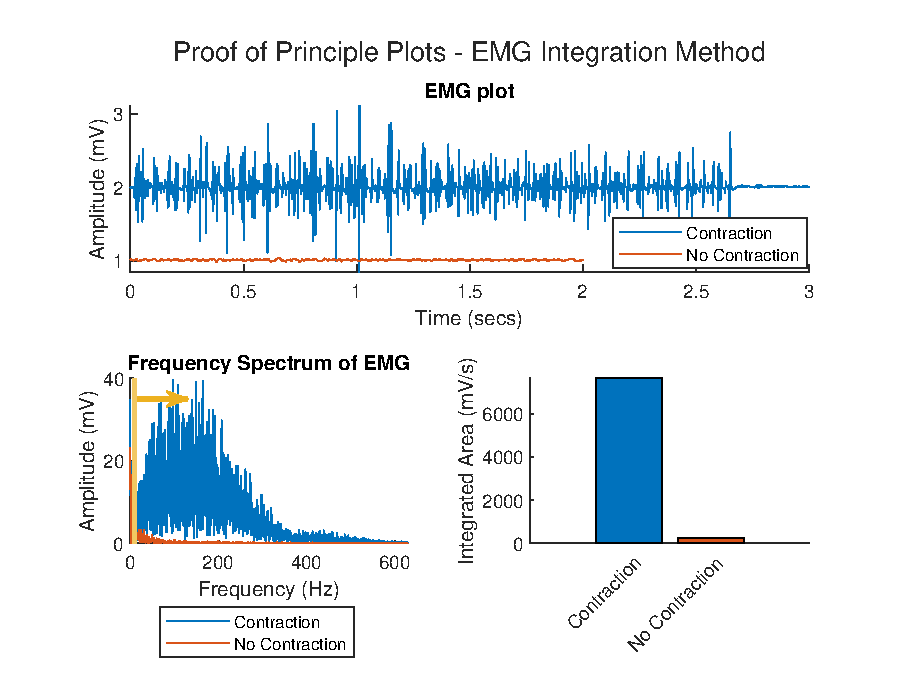
\includegraphics[width=0.75\linewidth]{figures/EMG_Proof_Of_Principle.eps}
    \caption{Plot Showing the Planned Analysis Method of EMG Data. a) Plot of extracted EMG data showing a sample during contraction (blue) and a sample where there is no contraction (orange). b) Plot of fourier transform of both samples above. The contraction sample has a significantly large amplitude in the 10-600Hz range. c) Integrated area of the fourier transforms in the 10-600Hz range. The difference in amplitudes can be clearly seen in this plot}
    \label{fig:EMG_Proof_of_principal}
\end{figure}

Unfortunately following the expansion of the method to the remainder of the task pilot phase data it was discovered that the alignment procedures did not function as intended. There was insufficient correlation between the triggers sent to the EMG software and the button strokes recorded in the behavioural data. This lack of correlation can be seen in figure \ref{fig:EMG_TrigComparisonB} where the expected file doesn't correlate in the slightest with any of the subjects behavioural data. The remainder of these comparison plots can be found in \ref{appendix:ExtraResults1_2}.
\begin{figure}[H]
    \centering
    \includegraphics[width=0.75\linewidth]{figures/EMG_Trigger_Comparison_b.eps}
    \caption{Recorded Triggers From the EMG Trace (Green) Compared to The Recorded Triggers From Each of the Subject's Trials (Orange)}
    \label{fig:EMG_TrigComparisonB}
\end{figure}